\documentclass[1p]{elsarticle_modified}
%\bibliographystyle{elsarticle-num}

%\usepackage[colorlinks]{hyperref}
%\usepackage{abbrmath_seonhwa} %\Abb, \Ascr, \Acal ,\Abf, \Afrak
\usepackage{amsfonts}
\usepackage{amssymb}
\usepackage{amsmath}
\usepackage{amsthm}
\usepackage{scalefnt}
\usepackage{amsbsy}
\usepackage{kotex}
\usepackage{caption}
\usepackage{subfig}
\usepackage{color}
\usepackage{graphicx}
\usepackage{xcolor} %% white, black, red, green, blue, cyan, magenta, yellow
\usepackage{float}
\usepackage{setspace}
\usepackage{hyperref}

\usepackage{tikz}
\usetikzlibrary{arrows}

\usepackage{multirow}
\usepackage{array} % fixed length table
\usepackage{hhline}

%%%%%%%%%%%%%%%%%%%%%
\makeatletter
\renewcommand*\env@matrix[1][\arraystretch]{%
	\edef\arraystretch{#1}%
	\hskip -\arraycolsep
	\let\@ifnextchar\new@ifnextchar
	\array{*\c@MaxMatrixCols c}}
\makeatother %https://tex.stackexchange.com/questions/14071/how-can-i-increase-the-line-spacing-in-a-matrix
%%%%%%%%%%%%%%%

\usepackage[normalem]{ulem}

\newcommand{\msout}[1]{\ifmmode\text{\sout{\ensuremath{#1}}}\else\sout{#1}\fi}
%SOURCE: \msout is \stkout macro in https://tex.stackexchange.com/questions/20609/strikeout-in-math-mode

\newcommand{\cancel}[1]{
	\ifmmode
	{\color{red}\msout{#1}}
	\else
	{\color{red}\sout{#1}}
	\fi
}

\newcommand{\add}[1]{
	{\color{blue}\uwave{#1}}
}

\newcommand{\replace}[2]{
	\ifmmode
	{\color{red}\msout{#1}}{\color{blue}\uwave{#2}}
	\else
	{\color{red}\sout{#1}}{\color{blue}\uwave{#2}}
	\fi
}

\newcommand{\Sol}{\mathcal{S}} %segment
\newcommand{\D}{D} %diagram
\newcommand{\A}{\mathcal{A}} %arc


%%%%%%%%%%%%%%%%%%%%%%%%%%%%%5 test

\def\sl{\operatorname{\textup{SL}}(2,\Cbb)}
\def\psl{\operatorname{\textup{PSL}}(2,\Cbb)}
\def\quan{\mkern 1mu \triangleright \mkern 1mu}

\theoremstyle{definition}
\newtheorem{thm}{Theorem}[section]
\newtheorem{prop}[thm]{Proposition}
\newtheorem{lem}[thm]{Lemma}
\newtheorem{ques}[thm]{Question}
\newtheorem{cor}[thm]{Corollary}
\newtheorem{defn}[thm]{Definition}
\newtheorem{exam}[thm]{Example}
\newtheorem{rmk}[thm]{Remark}
\newtheorem{alg}[thm]{Algorithm}

\newcommand{\I}{\sqrt{-1}}
\begin{document}

%\begin{frontmatter}
%
%\title{Boundary parabolic representations of knots up to 8 crossings}
%
%%% Group authors per affiliation:
%\author{Yunhi Cho} 
%\address{Department of Mathematics, University of Seoul, Seoul, Korea}
%\ead{yhcho@uos.ac.kr}
%
%
%\author{Seonhwa Kim} %\fnref{s_kim}}
%\address{Center for Geometry and Physics, Institute for Basic Science, Pohang, 37673, Korea}
%\ead{ryeona17@ibs.re.kr}
%
%\author{Hyuk Kim}
%\address{Department of Mathematical Sciences, Seoul National University, Seoul 08826, Korea}
%\ead{hyukkim@snu.ac.kr}
%
%\author{Seokbeom Yoon}
%\address{Department of Mathematical Sciences, Seoul National University, Seoul, 08826,  Korea}
%\ead{sbyoon15@snu.ac.kr}
%
%\begin{abstract}
%We find all boundary parabolic representation of knots up to 8 crossings.
%
%\end{abstract}
%\begin{keyword}
%    \MSC[2010] 57M25 
%\end{keyword}
%
%\end{frontmatter}

%\linenumbers
%\tableofcontents
%
\newcommand\colored[1]{\textcolor{white}{\rule[-0.35ex]{0.8em}{1.4ex}}\kern-0.8em\color{red} #1}%
%\newcommand\colored[1]{\textcolor{white}{ #1}\kern-2.17ex	\textcolor{white}{ #1}\kern-1.81ex	\textcolor{white}{ #1}\kern-2.15ex\color{red}#1	}

{\Large $\underline{12n_{0755}~(K12n_{0755})}$}

\setlength{\tabcolsep}{10pt}
\renewcommand{\arraystretch}{1.6}
\vspace{1cm}\begin{tabular}{m{100pt}>{\centering\arraybackslash}m{274pt}}
\multirow{5}{120pt}{
	\centering
	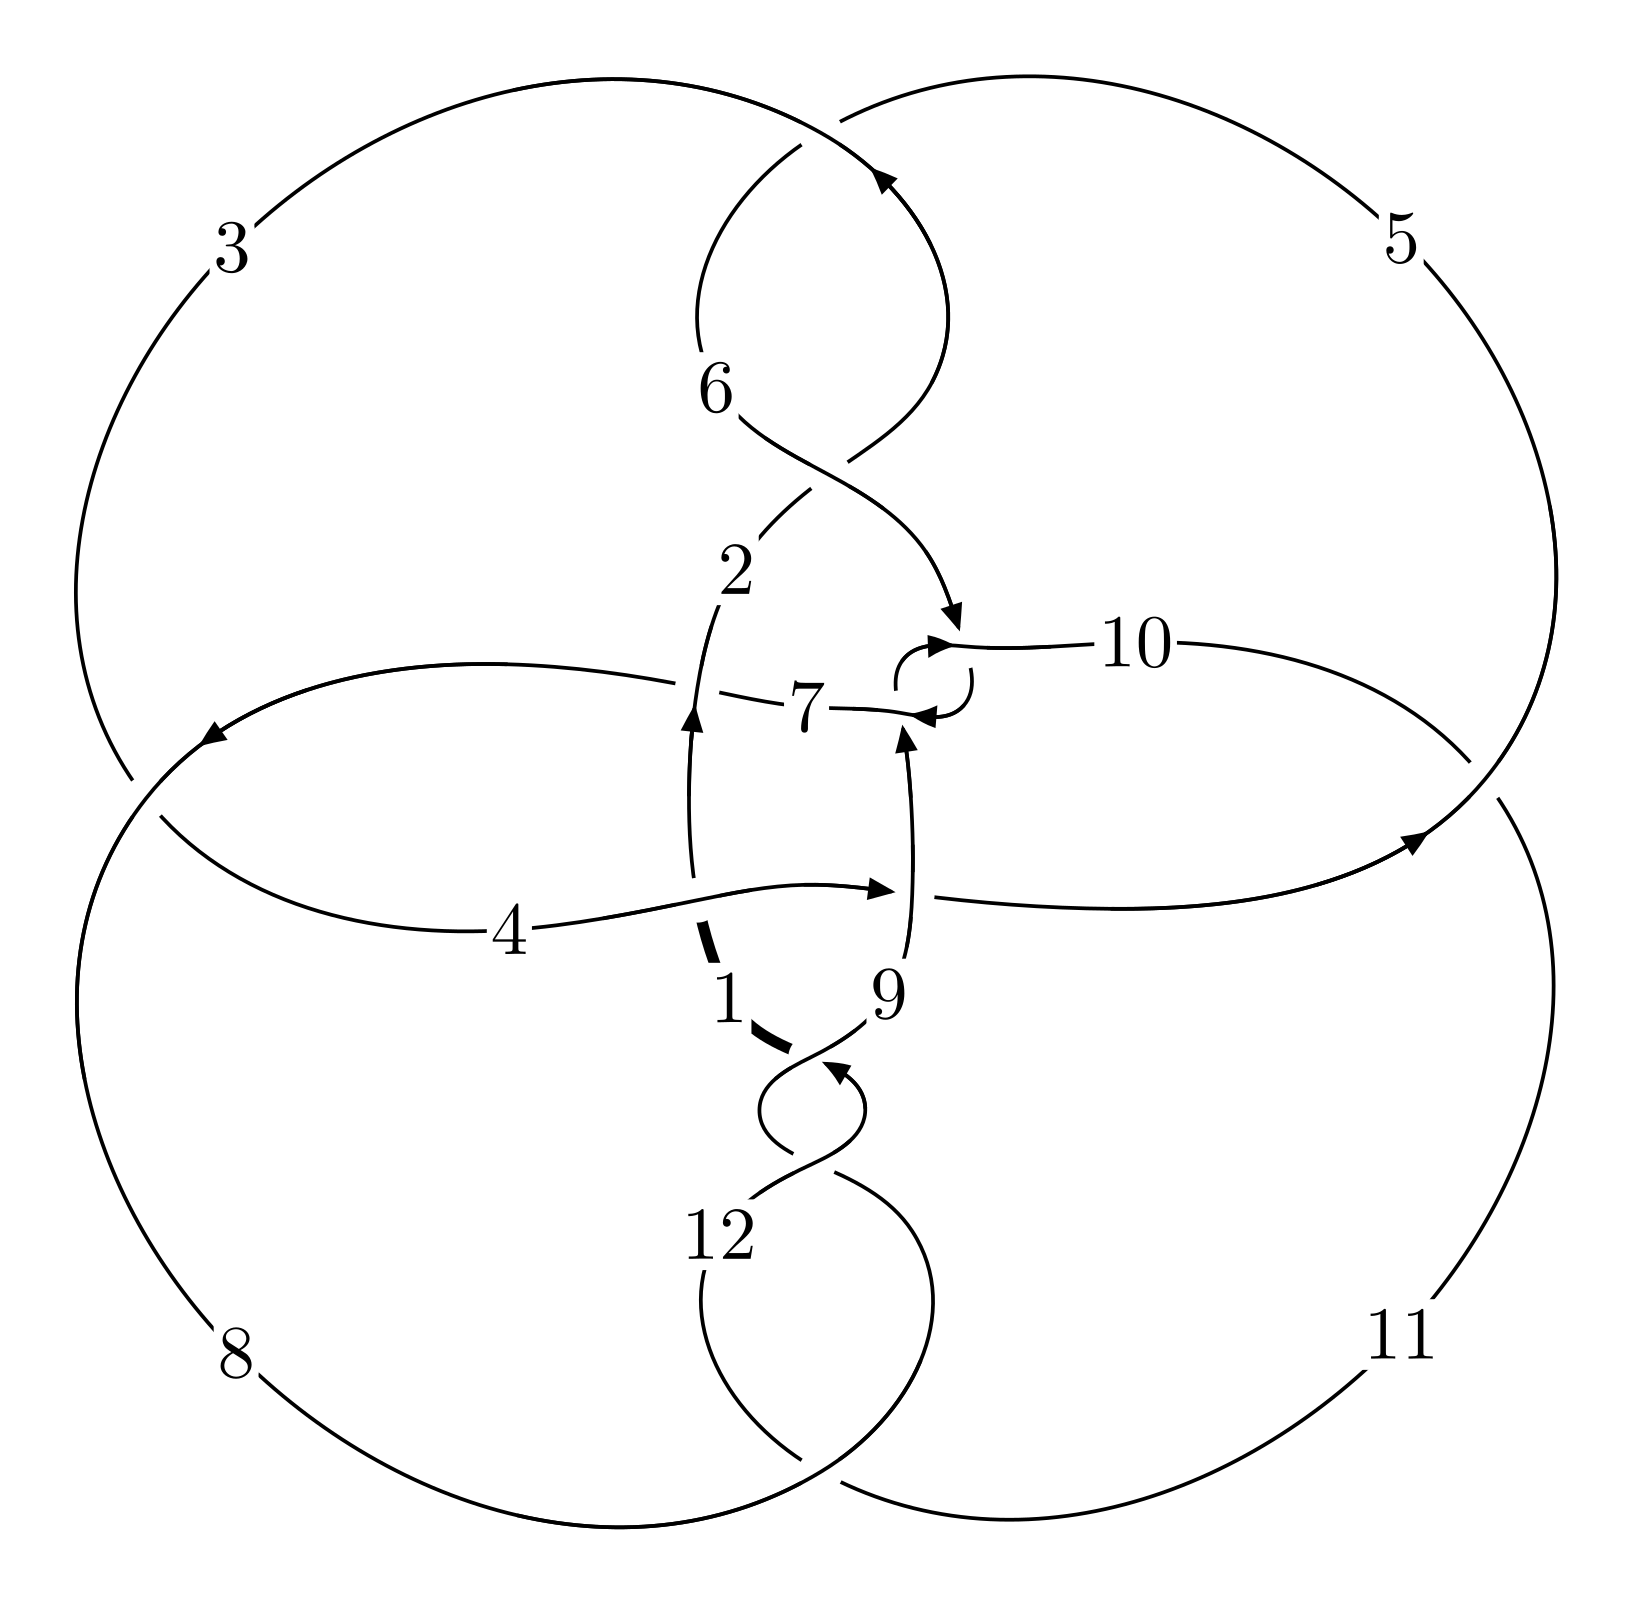
\includegraphics[width=112pt]{../../../GIT/diagram.site/Diagrams/png/2844_12n_0755.png}\\
\ \ \ A knot diagram\footnotemark}&
\allowdisplaybreaks
\textbf{Linearized knot diagam} \\
\cline{2-2}
 &
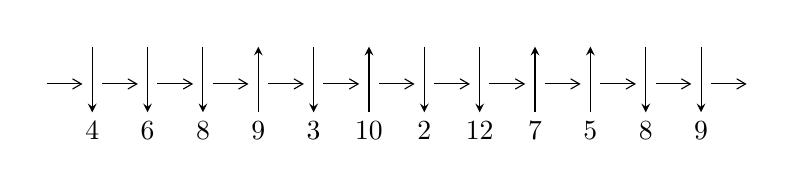
\begin{tikzpicture}[x=20pt, y=17pt]
	% nodes
	\node (C0) at (0, 0) {};
	\node (C1) at (1, 0) {};
	\node (C1U) at (1, +1) {};
	\node (C1D) at (1, -1) {4};

	\node (C2) at (2, 0) {};
	\node (C2U) at (2, +1) {};
	\node (C2D) at (2, -1) {6};

	\node (C3) at (3, 0) {};
	\node (C3U) at (3, +1) {};
	\node (C3D) at (3, -1) {8};

	\node (C4) at (4, 0) {};
	\node (C4U) at (4, +1) {};
	\node (C4D) at (4, -1) {9};

	\node (C5) at (5, 0) {};
	\node (C5U) at (5, +1) {};
	\node (C5D) at (5, -1) {3};

	\node (C6) at (6, 0) {};
	\node (C6U) at (6, +1) {};
	\node (C6D) at (6, -1) {10};

	\node (C7) at (7, 0) {};
	\node (C7U) at (7, +1) {};
	\node (C7D) at (7, -1) {2};

	\node (C8) at (8, 0) {};
	\node (C8U) at (8, +1) {};
	\node (C8D) at (8, -1) {12};

	\node (C9) at (9, 0) {};
	\node (C9U) at (9, +1) {};
	\node (C9D) at (9, -1) {7};

	\node (C10) at (10, 0) {};
	\node (C10U) at (10, +1) {};
	\node (C10D) at (10, -1) {5};

	\node (C11) at (11, 0) {};
	\node (C11U) at (11, +1) {};
	\node (C11D) at (11, -1) {8};

	\node (C12) at (12, 0) {};
	\node (C12U) at (12, +1) {};
	\node (C12D) at (12, -1) {9};
	\node (C13) at (13, 0) {};

	% arrows
	\draw[->,>={angle 60}]
	(C0) edge (C1) (C1) edge (C2) (C2) edge (C3) (C3) edge (C4) (C4) edge (C5) (C5) edge (C6) (C6) edge (C7) (C7) edge (C8) (C8) edge (C9) (C9) edge (C10) (C10) edge (C11) (C11) edge (C12) (C12) edge (C13) ;	\draw[->,>=stealth]
	(C1U) edge (C1D) (C2U) edge (C2D) (C3U) edge (C3D) (C4D) edge (C4U) (C5U) edge (C5D) (C6D) edge (C6U) (C7U) edge (C7D) (C8U) edge (C8D) (C9D) edge (C9U) (C10D) edge (C10U) (C11U) edge (C11D) (C12U) edge (C12D) ;
	\end{tikzpicture} \\
\hhline{~~} \\& 
\textbf{Solving Sequence} \\ \cline{2-2} 
 &
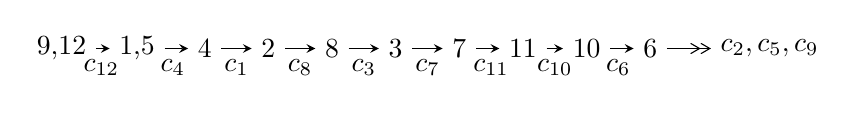
\begin{tikzpicture}[x=23pt, y=7pt]
	% node
	\node (A0) at (-1/8, 0) {9,12};
	\node (A1) at (17/16, 0) {1,5};
	\node (A2) at (17/8, 0) {4};
	\node (A3) at (25/8, 0) {2};
	\node (A4) at (33/8, 0) {8};
	\node (A5) at (41/8, 0) {3};
	\node (A6) at (49/8, 0) {7};
	\node (A7) at (57/8, 0) {11};
	\node (A8) at (65/8, 0) {10};
	\node (A9) at (73/8, 0) {6};
	\node (C1) at (1/2, -1) {$c_{12}$};
	\node (C2) at (13/8, -1) {$c_{4}$};
	\node (C3) at (21/8, -1) {$c_{1}$};
	\node (C4) at (29/8, -1) {$c_{8}$};
	\node (C5) at (37/8, -1) {$c_{3}$};
	\node (C6) at (45/8, -1) {$c_{7}$};
	\node (C7) at (53/8, -1) {$c_{11}$};
	\node (C8) at (61/8, -1) {$c_{10}$};
	\node (C9) at (69/8, -1) {$c_{6}$};
	\node (A10) at (11, 0) {$c_{2},c_{5},c_{9}$};

	% edge
	\draw[->,>=stealth]	
	(A0) edge (A1) (A1) edge (A2) (A2) edge (A3) (A3) edge (A4) (A4) edge (A5) (A5) edge (A6) (A6) edge (A7) (A7) edge (A8) (A8) edge (A9) ;
	\draw[->>,>={angle 60}]	
	(A9) edge (A10);
\end{tikzpicture} \\ 

\end{tabular} \\

\footnotetext{
The image of knot diagram is generated by the software ``\textbf{Draw programme}" developed by Andrew Bartholomew(\url{http://www.layer8.co.uk/maths/draw/index.htm\#Running-draw}), where we modified some parts for our purpose(\url{https://github.com/CATsTAILs/LinksPainter}).
}\phantom \\ \newline 
\centering \textbf{Ideals for irreducible components\footnotemark of $X_{\text{par}}$} 
 
\begin{align*}
I^u_{1}&=\langle 
1.18568\times10^{223} u^{81}+7.43164\times10^{223} u^{80}+\cdots+3.23988\times10^{222} b+4.31116\times10^{223},\\
\phantom{I^u_{1}}&\phantom{= \langle  }-1.92883\times10^{223} u^{81}-1.27832\times10^{224} u^{80}+\cdots+3.23988\times10^{222} a-1.11257\times10^{224},\\
\phantom{I^u_{1}}&\phantom{= \langle  }u^{82}+6 u^{81}+\cdots-11 u-3\rangle \\
I^u_{2}&=\langle 
-1890866592561 u^{22}+2410031480209 u^{21}+\cdots+3200805062239 b+12377780689946,\\
\phantom{I^u_{2}}&\phantom{= \langle  }-7028112561663 u^{22}+3451841046935 u^{21}+\cdots+3200805062239 a+16799928060287,\\
\phantom{I^u_{2}}&\phantom{= \langle  }u^{23}- u^{22}+\cdots-3 u+1\rangle \\
\\
\end{align*}
\raggedright * 2 irreducible components of $\dim_{\mathbb{C}}=0$, with total 105 representations.\\
\footnotetext{All coefficients of polynomials are rational numbers. But the coefficients are sometimes approximated in decimal forms when there is not enough margin.}
\newpage
\renewcommand{\arraystretch}{1}
\centering \section*{I. $I^u_{1}= \langle 1.19\times10^{223} u^{81}+7.43\times10^{223} u^{80}+\cdots+3.24\times10^{222} b+4.31\times10^{223},\;-1.93\times10^{223} u^{81}-1.28\times10^{224} u^{80}+\cdots+3.24\times10^{222} a-1.11\times10^{224},\;u^{82}+6 u^{81}+\cdots-11 u-3 \rangle$}
\flushleft \textbf{(i) Arc colorings}\\
\begin{tabular}{m{7pt} m{180pt} m{7pt} m{180pt} }
\flushright $a_{9}=$&$\begin{pmatrix}0\\u\end{pmatrix}$ \\
\flushright $a_{12}=$&$\begin{pmatrix}1\\0\end{pmatrix}$ \\
\flushright $a_{1}=$&$\begin{pmatrix}1\\u^2\end{pmatrix}$ \\
\flushright $a_{5}=$&$\begin{pmatrix}5.95340 u^{81}+39.4558 u^{80}+\cdots+211.539 u+34.3399\\-3.65962 u^{81}-22.9380 u^{80}+\cdots-108.880 u-13.3065\end{pmatrix}$ \\
\flushright $a_{4}=$&$\begin{pmatrix}5.95340 u^{81}+39.4558 u^{80}+\cdots+211.539 u+34.3399\\-2.25036 u^{81}-13.4360 u^{80}+\cdots-49.9298 u-2.10025\end{pmatrix}$ \\
\flushright $a_{2}=$&$\begin{pmatrix}2.45651 u^{81}+13.4972 u^{80}+\cdots+8.18878 u-15.0013\\3.58310 u^{81}+22.9490 u^{80}+\cdots+93.7957 u+10.9838\end{pmatrix}$ \\
\flushright $a_{8}=$&$\begin{pmatrix}u\\u\end{pmatrix}$ \\
\flushright $a_{3}=$&$\begin{pmatrix}4.36051 u^{81}+28.9039 u^{80}+\cdots+146.566 u+23.3322\\-3.84325 u^{81}-23.9879 u^{80}+\cdots-114.903 u-13.1080\end{pmatrix}$ \\
\flushright $a_{7}=$&$\begin{pmatrix}0.731709 u^{81}+7.25277 u^{80}+\cdots+134.322 u+45.5660\\-3.38808 u^{81}-21.7865 u^{80}+\cdots-116.411 u-20.2879\end{pmatrix}$ \\
\flushright $a_{11}=$&$\begin{pmatrix}- u^2+1\\- u^2\end{pmatrix}$ \\
\flushright $a_{10}=$&$\begin{pmatrix}1.23820 u^{81}+5.64993 u^{80}+\cdots-58.9501 u-27.1169\\2.72175 u^{81}+17.1903 u^{80}+\cdots+62.3171 u+5.29688\end{pmatrix}$ \\
\flushright $a_{6}=$&$\begin{pmatrix}1.96680 u^{81}+15.0496 u^{80}+\cdots+138.404 u+35.1527\\-4.97606 u^{81}-31.6255 u^{80}+\cdots-132.203 u-16.3332\end{pmatrix}$\\&\end{tabular}
\flushleft \textbf{(ii) Obstruction class $= -1$}\\~\\
\flushleft \textbf{(iii) Cusp Shapes $= -4.04743 u^{81}-27.0123 u^{80}+\cdots-215.823 u-51.0412$}\\~\\
\newpage\renewcommand{\arraystretch}{1}
\flushleft \textbf{(iv) u-Polynomials at the component}\newline \\
\begin{tabular}{m{50pt}|m{274pt}}
Crossings & \hspace{64pt}u-Polynomials at each crossing \\
\hline $$\begin{aligned}c_{1}\end{aligned}$$&$\begin{aligned}
&u^{82}-4 u^{81}+\cdots-14492 u+15032
\end{aligned}$\\
\hline $$\begin{aligned}c_{2},c_{5}\end{aligned}$$&$\begin{aligned}
&u^{82}-2 u^{81}+\cdots+386 u-21
\end{aligned}$\\
\hline $$\begin{aligned}c_{3}\end{aligned}$$&$\begin{aligned}
&u^{82}-2 u^{81}+\cdots-9468926 u-944291
\end{aligned}$\\
\hline $$\begin{aligned}c_{4}\end{aligned}$$&$\begin{aligned}
&u^{82}+u^{81}+\cdots+12069 u+3617
\end{aligned}$\\
\hline $$\begin{aligned}c_{6},c_{9}\end{aligned}$$&$\begin{aligned}
&u^{82}+u^{81}+\cdots+403 u+61
\end{aligned}$\\
\hline $$\begin{aligned}c_{7}\end{aligned}$$&$\begin{aligned}
&u^{82}+2 u^{81}+\cdots+28 u-151
\end{aligned}$\\
\hline $$\begin{aligned}c_{8},c_{11},c_{12}\end{aligned}$$&$\begin{aligned}
&u^{82}+6 u^{81}+\cdots-11 u-3
\end{aligned}$\\
\hline $$\begin{aligned}c_{10}\end{aligned}$$&$\begin{aligned}
&u^{82}- u^{81}+\cdots-2699225 u+632501
\end{aligned}$\\
\hline
\end{tabular}\\~\\
\newpage\renewcommand{\arraystretch}{1}
\flushleft \textbf{(v) Riley Polynomials at the component}\newline \\
\begin{tabular}{m{50pt}|m{274pt}}
Crossings & \hspace{64pt}Riley Polynomials at each crossing \\
\hline $$\begin{aligned}c_{1}\end{aligned}$$&$\begin{aligned}
&y^{82}+70 y^{81}+\cdots+3143561008 y+225961024
\end{aligned}$\\
\hline $$\begin{aligned}c_{2},c_{5}\end{aligned}$$&$\begin{aligned}
&y^{82}+52 y^{81}+\cdots-12412 y+441
\end{aligned}$\\
\hline $$\begin{aligned}c_{3}\end{aligned}$$&$\begin{aligned}
&y^{82}+48 y^{81}+\cdots-10989606497604 y+891685492681
\end{aligned}$\\
\hline $$\begin{aligned}c_{4}\end{aligned}$$&$\begin{aligned}
&y^{82}-71 y^{81}+\cdots-240578075 y+13082689
\end{aligned}$\\
\hline $$\begin{aligned}c_{6},c_{9}\end{aligned}$$&$\begin{aligned}
&y^{82}+47 y^{81}+\cdots+37305 y+3721
\end{aligned}$\\
\hline $$\begin{aligned}c_{7}\end{aligned}$$&$\begin{aligned}
&y^{82}+4 y^{81}+\cdots-246310 y+22801
\end{aligned}$\\
\hline $$\begin{aligned}c_{8},c_{11},c_{12}\end{aligned}$$&$\begin{aligned}
&y^{82}-18 y^{81}+\cdots-397 y+9
\end{aligned}$\\
\hline $$\begin{aligned}c_{10}\end{aligned}$$&$\begin{aligned}
&y^{82}-45 y^{81}+\cdots-21983555058121 y+400057515001
\end{aligned}$\\
\hline
\end{tabular}\\~\\
\newpage\flushleft \textbf{(vi) Complex Volumes and Cusp Shapes}
$$\begin{array}{c|c|c}  
\text{Solutions to }I^u_{1}& \I (\text{vol} + \sqrt{-1}CS) & \text{Cusp shape}\\
 \hline 
\begin{aligned}
u &= -0.806236 + 0.447979 I \\
a &= \phantom{-}0.116844 + 0.907734 I \\
b &= \phantom{-}0.313050 + 0.872682 I\end{aligned}
 & -0.042747 + 1.373590 I & \phantom{-0.000000 } 0 \\ \hline\begin{aligned}
u &= -0.806236 - 0.447979 I \\
a &= \phantom{-}0.116844 - 0.907734 I \\
b &= \phantom{-}0.313050 - 0.872682 I\end{aligned}
 & -0.042747 - 1.373590 I & \phantom{-0.000000 } 0 \\ \hline\begin{aligned}
u &= \phantom{-}0.835911 + 0.366396 I \\
a &= -0.895782 - 0.543357 I \\
b &= \phantom{-}0.686491 + 0.523534 I\end{aligned}
 & \phantom{-}1.47647 - 3.78347 I & \phantom{-0.000000 } 0 \\ \hline\begin{aligned}
u &= \phantom{-}0.835911 - 0.366396 I \\
a &= -0.895782 + 0.543357 I \\
b &= \phantom{-}0.686491 - 0.523534 I\end{aligned}
 & \phantom{-}1.47647 + 3.78347 I & \phantom{-0.000000 } 0 \\ \hline\begin{aligned}
u &= -0.701050 + 0.577627 I \\
a &= -0.094098 + 0.689287 I \\
b &= \phantom{-}0.443176 + 0.530379 I\end{aligned}
 & -0.048198 + 1.306660 I & \phantom{-0.000000 } 0 \\ \hline\begin{aligned}
u &= -0.701050 - 0.577627 I \\
a &= -0.094098 - 0.689287 I \\
b &= \phantom{-}0.443176 - 0.530379 I\end{aligned}
 & -0.048198 - 1.306660 I & \phantom{-0.000000 } 0 \\ \hline\begin{aligned}
u &= -0.874548 + 0.018157 I \\
a &= -1.53808 + 0.49342 I \\
b &= \phantom{-}1.016920 - 0.505156 I\end{aligned}
 & -1.58786 + 5.67587 I & -9.37818 - 5.48357 I \\ \hline\begin{aligned}
u &= -0.874548 - 0.018157 I \\
a &= -1.53808 - 0.49342 I \\
b &= \phantom{-}1.016920 + 0.505156 I\end{aligned}
 & -1.58786 - 5.67587 I & -9.37818 + 5.48357 I \\ \hline\begin{aligned}
u &= -1.15383\phantom{ +0.000000I} \\
a &= -0.365134\phantom{ +0.000000I} \\
b &= -0.413477\phantom{ +0.000000I}\end{aligned}
 & -2.52087\phantom{ +0.000000I} & \phantom{-0.000000 } 0 \\ \hline\begin{aligned}
u &= -0.750355 + 0.898180 I \\
a &= -0.25763 - 1.49046 I \\
b &= \phantom{-}0.73558 - 1.48679 I\end{aligned}
 & \phantom{-}7.24531 + 4.47737 I & \phantom{-0.000000 } 0\\
 \hline 
 \end{array}$$\newpage$$\begin{array}{c|c|c}  
\text{Solutions to }I^u_{1}& \I (\text{vol} + \sqrt{-1}CS) & \text{Cusp shape}\\
 \hline 
\begin{aligned}
u &= -0.750355 - 0.898180 I \\
a &= -0.25763 + 1.49046 I \\
b &= \phantom{-}0.73558 + 1.48679 I\end{aligned}
 & \phantom{-}7.24531 - 4.47737 I & \phantom{-0.000000 } 0 \\ \hline\begin{aligned}
u &= -0.425248 + 1.099560 I \\
a &= \phantom{-}0.45745 + 1.56142 I \\
b &= -0.381257 + 0.936714 I\end{aligned}
 & \phantom{-}3.38750 + 5.56328 I & \phantom{-0.000000 } 0 \\ \hline\begin{aligned}
u &= -0.425248 - 1.099560 I \\
a &= \phantom{-}0.45745 - 1.56142 I \\
b &= -0.381257 - 0.936714 I\end{aligned}
 & \phantom{-}3.38750 - 5.56328 I & \phantom{-0.000000 } 0 \\ \hline\begin{aligned}
u &= -0.821348 + 0.914226 I \\
a &= -0.931141 - 0.836821 I \\
b &= -0.24212 - 1.51037 I\end{aligned}
 & \phantom{-}2.05800 - 4.23861 I & \phantom{-0.000000 } 0 \\ \hline\begin{aligned}
u &= -0.821348 - 0.914226 I \\
a &= -0.931141 + 0.836821 I \\
b &= -0.24212 + 1.51037 I\end{aligned}
 & \phantom{-}2.05800 + 4.23861 I & \phantom{-0.000000 } 0 \\ \hline\begin{aligned}
u &= \phantom{-}0.822864 + 0.959472 I \\
a &= -0.58005 + 1.29619 I \\
b &= \phantom{-}0.60803 + 1.79418 I\end{aligned}
 & \phantom{-}7.49350 - 0.72833 I & \phantom{-0.000000 } 0 \\ \hline\begin{aligned}
u &= \phantom{-}0.822864 - 0.959472 I \\
a &= -0.58005 - 1.29619 I \\
b &= \phantom{-}0.60803 - 1.79418 I\end{aligned}
 & \phantom{-}7.49350 + 0.72833 I & \phantom{-0.000000 } 0 \\ \hline\begin{aligned}
u &= -0.673993 + 0.279521 I \\
a &= -0.540764 + 0.727882 I \\
b &= -1.64438 + 0.06585 I\end{aligned}
 & -3.58880 + 2.02013 I & -13.3165 - 8.2924 I \\ \hline\begin{aligned}
u &= -0.673993 - 0.279521 I \\
a &= -0.540764 - 0.727882 I \\
b &= -1.64438 - 0.06585 I\end{aligned}
 & -3.58880 - 2.02013 I & -13.3165 + 8.2924 I \\ \hline\begin{aligned}
u &= \phantom{-}0.883514 + 0.916466 I \\
a &= -0.822379 + 0.907210 I \\
b &= \phantom{-}0.16986 + 1.49068 I\end{aligned}
 & \phantom{-}4.92220 - 0.58301 I & \phantom{-0.000000 } 0\\
 \hline 
 \end{array}$$\newpage$$\begin{array}{c|c|c}  
\text{Solutions to }I^u_{1}& \I (\text{vol} + \sqrt{-1}CS) & \text{Cusp shape}\\
 \hline 
\begin{aligned}
u &= \phantom{-}0.883514 - 0.916466 I \\
a &= -0.822379 - 0.907210 I \\
b &= \phantom{-}0.16986 - 1.49068 I\end{aligned}
 & \phantom{-}4.92220 + 0.58301 I & \phantom{-0.000000 } 0 \\ \hline\begin{aligned}
u &= -0.631826 + 0.348866 I \\
a &= \phantom{-}0.61391 + 2.12275 I \\
b &= -1.108410 + 0.201294 I\end{aligned}
 & -3.40457 + 0.57973 I & -9.43437 - 4.19864 I \\ \hline\begin{aligned}
u &= -0.631826 - 0.348866 I \\
a &= \phantom{-}0.61391 - 2.12275 I \\
b &= -1.108410 - 0.201294 I\end{aligned}
 & -3.40457 - 0.57973 I & -9.43437 + 4.19864 I \\ \hline\begin{aligned}
u &= \phantom{-}0.712432 + 0.084214 I \\
a &= \phantom{-}0.58489 - 1.49460 I \\
b &= \phantom{-}0.40860 - 1.43638 I\end{aligned}
 & -1.50757 - 6.70450 I & -11.21324 + 6.26401 I \\ \hline\begin{aligned}
u &= \phantom{-}0.712432 - 0.084214 I \\
a &= \phantom{-}0.58489 + 1.49460 I \\
b &= \phantom{-}0.40860 + 1.43638 I\end{aligned}
 & -1.50757 + 6.70450 I & -11.21324 - 6.26401 I \\ \hline\begin{aligned}
u &= -0.450661 + 0.549059 I \\
a &= \phantom{-}0.283735 - 0.371733 I \\
b &= \phantom{-}1.99582 + 0.12483 I\end{aligned}
 & \phantom{-}0.42096 + 8.02120 I & -2.11051 - 11.91858 I \\ \hline\begin{aligned}
u &= -0.450661 - 0.549059 I \\
a &= \phantom{-}0.283735 + 0.371733 I \\
b &= \phantom{-}1.99582 - 0.12483 I\end{aligned}
 & \phantom{-}0.42096 - 8.02120 I & -2.11051 + 11.91858 I \\ \hline\begin{aligned}
u &= -0.974900 + 0.848966 I \\
a &= -0.773538 - 0.899541 I \\
b &= \phantom{-}0.564453 - 1.073860 I\end{aligned}
 & \phantom{-}0.47523 + 4.56353 I & \phantom{-0.000000 } 0 \\ \hline\begin{aligned}
u &= -0.974900 - 0.848966 I \\
a &= -0.773538 + 0.899541 I \\
b &= \phantom{-}0.564453 + 1.073860 I\end{aligned}
 & \phantom{-}0.47523 - 4.56353 I & \phantom{-0.000000 } 0 \\ \hline\begin{aligned}
u &= -0.950851 + 0.883034 I \\
a &= \phantom{-}0.330778 + 0.966106 I \\
b &= -0.132030 + 1.199490 I\end{aligned}
 & \phantom{-}0.53361 + 1.91658 I & \phantom{-0.000000 } 0\\
 \hline 
 \end{array}$$\newpage$$\begin{array}{c|c|c}  
\text{Solutions to }I^u_{1}& \I (\text{vol} + \sqrt{-1}CS) & \text{Cusp shape}\\
 \hline 
\begin{aligned}
u &= -0.950851 - 0.883034 I \\
a &= \phantom{-}0.330778 - 0.966106 I \\
b &= -0.132030 - 1.199490 I\end{aligned}
 & \phantom{-}0.53361 - 1.91658 I & \phantom{-0.000000 } 0 \\ \hline\begin{aligned}
u &= -0.065661 + 0.689575 I \\
a &= \phantom{-}0.188975 - 0.904470 I \\
b &= -0.618127 + 0.219610 I\end{aligned}
 & \phantom{-}0.90992 + 2.47162 I & -2.89492 - 3.06151 I \\ \hline\begin{aligned}
u &= -0.065661 - 0.689575 I \\
a &= \phantom{-}0.188975 + 0.904470 I \\
b &= -0.618127 - 0.219610 I\end{aligned}
 & \phantom{-}0.90992 - 2.47162 I & -2.89492 + 3.06151 I \\ \hline\begin{aligned}
u &= -0.582300 + 1.190720 I \\
a &= -0.159473 - 0.797913 I \\
b &= \phantom{-}0.03486 - 1.72869 I\end{aligned}
 & \phantom{-}6.45996 + 1.18643 I & \phantom{-0.000000 } 0 \\ \hline\begin{aligned}
u &= -0.582300 - 1.190720 I \\
a &= -0.159473 + 0.797913 I \\
b &= \phantom{-}0.03486 + 1.72869 I\end{aligned}
 & \phantom{-}6.45996 - 1.18643 I & \phantom{-0.000000 } 0 \\ \hline\begin{aligned}
u &= -1.098680 + 0.754147 I \\
a &= \phantom{-}1.002280 + 0.473388 I \\
b &= \phantom{-}0.219617 + 1.329070 I\end{aligned}
 & \phantom{-}6.12437 + 1.73968 I & \phantom{-0.000000 } 0 \\ \hline\begin{aligned}
u &= -1.098680 - 0.754147 I \\
a &= \phantom{-}1.002280 - 0.473388 I \\
b &= \phantom{-}0.219617 - 1.329070 I\end{aligned}
 & \phantom{-}6.12437 - 1.73968 I & \phantom{-0.000000 } 0 \\ \hline\begin{aligned}
u &= -0.260067 + 0.609056 I \\
a &= \phantom{-}1.90359 - 0.34249 I \\
b &= -0.049741 - 0.351548 I\end{aligned}
 & \phantom{-}3.81108 + 2.73141 I & \phantom{-}4.36589 - 2.14562 I \\ \hline\begin{aligned}
u &= -0.260067 - 0.609056 I \\
a &= \phantom{-}1.90359 + 0.34249 I \\
b &= -0.049741 + 0.351548 I\end{aligned}
 & \phantom{-}3.81108 - 2.73141 I & \phantom{-}4.36589 + 2.14562 I \\ \hline\begin{aligned}
u &= -1.018490 + 0.869250 I \\
a &= \phantom{-}0.60257 + 1.28317 I \\
b &= -0.78229 + 1.66142 I\end{aligned}
 & \phantom{-}1.48594 + 10.83750 I & \phantom{-0.000000 } 0\\
 \hline 
 \end{array}$$\newpage$$\begin{array}{c|c|c}  
\text{Solutions to }I^u_{1}& \I (\text{vol} + \sqrt{-1}CS) & \text{Cusp shape}\\
 \hline 
\begin{aligned}
u &= -1.018490 - 0.869250 I \\
a &= \phantom{-}0.60257 - 1.28317 I \\
b &= -0.78229 - 1.66142 I\end{aligned}
 & \phantom{-}1.48594 - 10.83750 I & \phantom{-0.000000 } 0 \\ \hline\begin{aligned}
u &= \phantom{-}1.005000 + 0.889070 I \\
a &= \phantom{-}0.603105 - 1.085290 I \\
b &= -0.46354 - 1.66659 I\end{aligned}
 & \phantom{-}4.55738 - 6.10859 I & \phantom{-0.000000 } 0 \\ \hline\begin{aligned}
u &= \phantom{-}1.005000 - 0.889070 I \\
a &= \phantom{-}0.603105 + 1.085290 I \\
b &= -0.46354 + 1.66659 I\end{aligned}
 & \phantom{-}4.55738 + 6.10859 I & \phantom{-0.000000 } 0 \\ \hline\begin{aligned}
u &= \phantom{-}0.520783 + 0.400279 I \\
a &= -0.419662 + 0.443731 I \\
b &= \phantom{-}1.48234 + 0.41015 I\end{aligned}
 & \phantom{-}2.58165 - 3.80058 I & \phantom{-}2.24184 + 7.84876 I \\ \hline\begin{aligned}
u &= \phantom{-}0.520783 - 0.400279 I \\
a &= -0.419662 - 0.443731 I \\
b &= \phantom{-}1.48234 - 0.41015 I\end{aligned}
 & \phantom{-}2.58165 + 3.80058 I & \phantom{-}2.24184 - 7.84876 I \\ \hline\begin{aligned}
u &= \phantom{-}0.626125 + 0.145468 I \\
a &= -0.18087 - 2.79944 I \\
b &= -0.587182 + 0.101724 I\end{aligned}
 & -4.14051 - 1.50707 I & -13.3689 + 5.4539 I \\ \hline\begin{aligned}
u &= \phantom{-}0.626125 - 0.145468 I \\
a &= -0.18087 + 2.79944 I \\
b &= -0.587182 - 0.101724 I\end{aligned}
 & -4.14051 + 1.50707 I & -13.3689 - 5.4539 I \\ \hline\begin{aligned}
u &= \phantom{-}1.063340 + 0.849536 I \\
a &= \phantom{-}0.956780 - 0.757979 I \\
b &= -0.03841 - 1.76406 I\end{aligned}
 & \phantom{-}6.72056 - 5.96162 I & \phantom{-0.000000 } 0 \\ \hline\begin{aligned}
u &= \phantom{-}1.063340 - 0.849536 I \\
a &= \phantom{-}0.956780 + 0.757979 I \\
b &= -0.03841 + 1.76406 I\end{aligned}
 & \phantom{-}6.72056 + 5.96162 I & \phantom{-0.000000 } 0 \\ \hline\begin{aligned}
u &= \phantom{-}0.476810 + 0.402159 I \\
a &= \phantom{-}2.10026 + 2.83473 I \\
b &= \phantom{-}0.284676 + 0.060377 I\end{aligned}
 & -0.29800 - 7.98807 I & -3.3717 + 15.3963 I\\
 \hline 
 \end{array}$$\newpage$$\begin{array}{c|c|c}  
\text{Solutions to }I^u_{1}& \I (\text{vol} + \sqrt{-1}CS) & \text{Cusp shape}\\
 \hline 
\begin{aligned}
u &= \phantom{-}0.476810 - 0.402159 I \\
a &= \phantom{-}2.10026 - 2.83473 I \\
b &= \phantom{-}0.284676 - 0.060377 I\end{aligned}
 & -0.29800 + 7.98807 I & -3.3717 - 15.3963 I \\ \hline\begin{aligned}
u &= -0.387572 + 0.483892 I \\
a &= -0.506786 + 0.595374 I \\
b &= \phantom{-}0.161400 + 0.343252 I\end{aligned}
 & -0.209152 + 1.137760 I & -2.77451 - 5.70461 I \\ \hline\begin{aligned}
u &= -0.387572 - 0.483892 I \\
a &= -0.506786 - 0.595374 I \\
b &= \phantom{-}0.161400 - 0.343252 I\end{aligned}
 & -0.209152 - 1.137760 I & -2.77451 + 5.70461 I \\ \hline\begin{aligned}
u &= \phantom{-}0.557426 + 0.231728 I \\
a &= -0.33867 - 1.76399 I \\
b &= -1.10016 - 1.23923 I\end{aligned}
 & -3.82873 - 0.00668 I & -16.1459 + 7.0292 I \\ \hline\begin{aligned}
u &= \phantom{-}0.557426 - 0.231728 I \\
a &= -0.33867 + 1.76399 I \\
b &= -1.10016 + 1.23923 I\end{aligned}
 & -3.82873 + 0.00668 I & -16.1459 - 7.0292 I \\ \hline\begin{aligned}
u &= \phantom{-}1.409430 + 0.115816 I \\
a &= -0.164334 + 0.187390 I \\
b &= -0.135012 - 0.469782 I\end{aligned}
 & -6.54986 - 3.23861 I & \phantom{-0.000000 } 0 \\ \hline\begin{aligned}
u &= \phantom{-}1.409430 - 0.115816 I \\
a &= -0.164334 - 0.187390 I \\
b &= -0.135012 + 0.469782 I\end{aligned}
 & -6.54986 + 3.23861 I & \phantom{-0.000000 } 0 \\ \hline\begin{aligned}
u &= \phantom{-}0.84939 + 1.16040 I \\
a &= \phantom{-}0.631650 - 0.921823 I \\
b &= \phantom{-}0.03685 - 1.45118 I\end{aligned}
 & \phantom{-}9.67520 + 3.07500 I & \phantom{-0.000000 } 0 \\ \hline\begin{aligned}
u &= \phantom{-}0.84939 - 1.16040 I \\
a &= \phantom{-}0.631650 + 0.921823 I \\
b &= \phantom{-}0.03685 + 1.45118 I\end{aligned}
 & \phantom{-}9.67520 - 3.07500 I & \phantom{-0.000000 } 0 \\ \hline\begin{aligned}
u &= -0.98461 + 1.06132 I \\
a &= -0.518913 - 1.125470 I \\
b &= \phantom{-}0.359482 - 1.003890 I\end{aligned}
 & \phantom{-}0.93021 + 4.88868 I & \phantom{-0.000000 } 0\\
 \hline 
 \end{array}$$\newpage$$\begin{array}{c|c|c}  
\text{Solutions to }I^u_{1}& \I (\text{vol} + \sqrt{-1}CS) & \text{Cusp shape}\\
 \hline 
\begin{aligned}
u &= -0.98461 - 1.06132 I \\
a &= -0.518913 + 1.125470 I \\
b &= \phantom{-}0.359482 + 1.003890 I\end{aligned}
 & \phantom{-}0.93021 - 4.88868 I & \phantom{-0.000000 } 0 \\ \hline\begin{aligned}
u &= -0.86125 + 1.16514 I \\
a &= \phantom{-}0.705142 + 0.791235 I \\
b &= \phantom{-}0.19060 + 1.59932 I\end{aligned}
 & \phantom{-}6.48875 - 9.64645 I & \phantom{-0.000000 } 0 \\ \hline\begin{aligned}
u &= -0.86125 - 1.16514 I \\
a &= \phantom{-}0.705142 - 0.791235 I \\
b &= \phantom{-}0.19060 - 1.59932 I\end{aligned}
 & \phantom{-}6.48875 + 9.64645 I & \phantom{-0.000000 } 0 \\ \hline\begin{aligned}
u &= \phantom{-}0.82211 + 1.22177 I \\
a &= -0.397179 + 0.816867 I \\
b &= \phantom{-}0.40067 + 1.95196 I\end{aligned}
 & \phantom{-}6.25873 - 3.82475 I & \phantom{-0.000000 } 0 \\ \hline\begin{aligned}
u &= \phantom{-}0.82211 - 1.22177 I \\
a &= -0.397179 - 0.816867 I \\
b &= \phantom{-}0.40067 - 1.95196 I\end{aligned}
 & \phantom{-}6.25873 + 3.82475 I & \phantom{-0.000000 } 0 \\ \hline\begin{aligned}
u &= \phantom{-}0.510704 + 0.080688 I \\
a &= -1.91916 + 0.40206 I \\
b &= \phantom{-}0.714917 + 0.882843 I\end{aligned}
 & \phantom{-}2.50196 - 2.66858 I & -1.26207 + 3.93369 I \\ \hline\begin{aligned}
u &= \phantom{-}0.510704 - 0.080688 I \\
a &= -1.91916 - 0.40206 I \\
b &= \phantom{-}0.714917 - 0.882843 I\end{aligned}
 & \phantom{-}2.50196 + 2.66858 I & -1.26207 - 3.93369 I \\ \hline\begin{aligned}
u &= -1.13264 + 0.96131 I \\
a &= -0.573896 - 1.114140 I \\
b &= \phantom{-}0.77313 - 1.68807 I\end{aligned}
 & \phantom{-}5.5638 + 17.2835 I & \phantom{-0.000000 } 0 \\ \hline\begin{aligned}
u &= -1.13264 - 0.96131 I \\
a &= -0.573896 + 1.114140 I \\
b &= \phantom{-}0.77313 + 1.68807 I\end{aligned}
 & \phantom{-}5.5638 - 17.2835 I & \phantom{-0.000000 } 0 \\ \hline\begin{aligned}
u &= \phantom{-}1.13751 + 0.96101 I \\
a &= -0.573662 + 1.059270 I \\
b &= \phantom{-}0.54430 + 1.58374 I\end{aligned}
 & \phantom{-}8.71424 - 10.69960 I & \phantom{-0.000000 } 0\\
 \hline 
 \end{array}$$\newpage$$\begin{array}{c|c|c}  
\text{Solutions to }I^u_{1}& \I (\text{vol} + \sqrt{-1}CS) & \text{Cusp shape}\\
 \hline 
\begin{aligned}
u &= \phantom{-}1.13751 - 0.96101 I \\
a &= -0.573662 - 1.059270 I \\
b &= \phantom{-}0.54430 - 1.58374 I\end{aligned}
 & \phantom{-}8.71424 + 10.69960 I & \phantom{-0.000000 } 0 \\ \hline\begin{aligned}
u &= -1.48390 + 0.24377 I \\
a &= -0.031323 - 0.358276 I \\
b &= -0.235266 - 0.710195 I\end{aligned}
 & -1.098920 + 0.366529 I & \phantom{-0.000000 } 0 \\ \hline\begin{aligned}
u &= -1.48390 - 0.24377 I \\
a &= -0.031323 + 0.358276 I \\
b &= -0.235266 + 0.710195 I\end{aligned}
 & -1.098920 - 0.366529 I & \phantom{-0.000000 } 0 \\ \hline\begin{aligned}
u &= \phantom{-}0.492926\phantom{ +0.000000I} \\
a &= \phantom{-}1.00800\phantom{ +0.000000I} \\
b &= -1.10716\phantom{ +0.000000I}\end{aligned}
 & -1.69272\phantom{ +0.000000I} & -3.43940\phantom{ +0.000000I} \\ \hline\begin{aligned}
u &= \phantom{-}1.11375 + 1.03431 I \\
a &= \phantom{-}0.577088 - 0.734092 I \\
b &= -0.56145 - 1.82423 I\end{aligned}
 & \phantom{-}5.35450 - 4.18150 I & \phantom{-0.000000 } 0 \\ \hline\begin{aligned}
u &= \phantom{-}1.11375 - 1.03431 I \\
a &= \phantom{-}0.577088 + 0.734092 I \\
b &= -0.56145 + 1.82423 I\end{aligned}
 & \phantom{-}5.35450 + 4.18150 I & \phantom{-0.000000 } 0 \\ \hline\begin{aligned}
u &= \phantom{-}1.54442 + 0.24643 I \\
a &= \phantom{-}0.217680 + 0.007983 I \\
b &= -0.345847 + 0.430990 I\end{aligned}
 & -4.74804 - 6.73053 I & \phantom{-0.000000 } 0 \\ \hline\begin{aligned}
u &= \phantom{-}1.54442 - 0.24643 I \\
a &= \phantom{-}0.217680 - 0.007983 I \\
b &= -0.345847 - 0.430990 I\end{aligned}
 & -4.74804 + 6.73053 I & \phantom{-0.000000 } 0 \\ \hline\begin{aligned}
u &= -1.28649 + 0.97876 I \\
a &= \phantom{-}0.566181 + 0.565715 I \\
b &= -0.75720 + 1.37954 I\end{aligned}
 & \phantom{-}4.36428 + 6.64097 I & \phantom{-0.000000 } 0 \\ \hline\begin{aligned}
u &= -1.28649 - 0.97876 I \\
a &= \phantom{-}0.566181 - 0.565715 I \\
b &= -0.75720 - 1.37954 I\end{aligned}
 & \phantom{-}4.36428 - 6.64097 I & \phantom{-0.000000 } 0\\
 \hline 
 \end{array}$$\newpage$$\begin{array}{c|c|c}  
\text{Solutions to }I^u_{1}& \I (\text{vol} + \sqrt{-1}CS) & \text{Cusp shape}\\
 \hline 
\begin{aligned}
u &= -0.338398 + 0.065785 I \\
a &= -3.21361 + 0.05803 I \\
b &= -0.202094 + 0.875685 I\end{aligned}
 & \phantom{-}0.77876 + 2.17059 I & -3.05306 - 2.50525 I \\ \hline\begin{aligned}
u &= -0.338398 - 0.065785 I \\
a &= -3.21361 - 0.05803 I \\
b &= -0.202094 - 0.875685 I\end{aligned}
 & \phantom{-}0.77876 - 2.17059 I & -3.05306 + 2.50525 I\\
 \hline 
 \end{array}$$\newpage\newpage\renewcommand{\arraystretch}{1}
\centering \section*{II. $I^u_{2}= \langle -1.89\times10^{12} u^{22}+2.41\times10^{12} u^{21}+\cdots+3.20\times10^{12} b+1.24\times10^{13},\;-7.03\times10^{12} u^{22}+3.45\times10^{12} u^{21}+\cdots+3.20\times10^{12} a+1.68\times10^{13},\;u^{23}- u^{22}+\cdots-3 u+1 \rangle$}
\flushleft \textbf{(i) Arc colorings}\\
\begin{tabular}{m{7pt} m{180pt} m{7pt} m{180pt} }
\flushright $a_{9}=$&$\begin{pmatrix}0\\u\end{pmatrix}$ \\
\flushright $a_{12}=$&$\begin{pmatrix}1\\0\end{pmatrix}$ \\
\flushright $a_{1}=$&$\begin{pmatrix}1\\u^2\end{pmatrix}$ \\
\flushright $a_{5}=$&$\begin{pmatrix}2.19573 u^{22}-1.07843 u^{21}+\cdots+7.61282 u-5.24866\\0.590747 u^{22}-0.752945 u^{21}+\cdots+2.18120 u-3.86708\end{pmatrix}$ \\
\flushright $a_{4}=$&$\begin{pmatrix}2.19573 u^{22}-1.07843 u^{21}+\cdots+7.61282 u-5.24866\\0.977901 u^{22}-0.852039 u^{21}+\cdots+3.33738 u-4.98439\end{pmatrix}$ \\
\flushright $a_{2}=$&$\begin{pmatrix}-4.02910 u^{22}+1.11016 u^{21}+\cdots-18.5602 u+6.75980\\-3.12743 u^{22}+1.87545 u^{21}+\cdots-8.95195 u+6.59751\end{pmatrix}$ \\
\flushright $a_{8}=$&$\begin{pmatrix}u\\u\end{pmatrix}$ \\
\flushright $a_{3}=$&$\begin{pmatrix}1.84688 u^{22}-1.23642 u^{21}+\cdots+5.85633 u-4.25721\\0.629049 u^{22}-1.01003 u^{21}+\cdots+1.58088 u-3.99294\end{pmatrix}$ \\
\flushright $a_{7}=$&$\begin{pmatrix}4.27517 u^{22}-1.90167 u^{21}+\cdots+10.9963 u-7.43747\\0.325782 u^{22}+0.886134 u^{21}+\cdots+7.99290 u-4.83426\end{pmatrix}$ \\
\flushright $a_{11}=$&$\begin{pmatrix}- u^2+1\\- u^2\end{pmatrix}$ \\
\flushright $a_{10}=$&$\begin{pmatrix}-2.56863 u^{22}+0.695455 u^{21}+\cdots-13.1510 u+1.06396\\-2.57971 u^{22}+1.28620 u^{21}+\cdots-9.48726 u+5.94213\end{pmatrix}$ \\
\flushright $a_{6}=$&$\begin{pmatrix}-0.598057 u^{22}+1.30233 u^{21}+\cdots+4.71204 u+5.08438\\1.69862 u^{22}+0.393112 u^{21}+\cdots+15.8887 u-6.69634\end{pmatrix}$\\&\end{tabular}
\flushleft \textbf{(ii) Obstruction class $= 1$}\\~\\
\flushleft \textbf{(iii) Cusp Shapes $= \frac{36632544074525}{3200805062239} u^{22}-\frac{23085135423462}{3200805062239} u^{21}+\cdots+\frac{89601441698510}{3200805062239} u-\frac{81515705395485}{3200805062239}$}\\~\\
\newpage\renewcommand{\arraystretch}{1}
\flushleft \textbf{(iv) u-Polynomials at the component}\newline \\
\begin{tabular}{m{50pt}|m{274pt}}
Crossings & \hspace{64pt}u-Polynomials at each crossing \\
\hline $$\begin{aligned}c_{1}\end{aligned}$$&$\begin{aligned}
&u^{23}- u^{22}+\cdots+4 u^2-1
\end{aligned}$\\
\hline $$\begin{aligned}c_{2}\end{aligned}$$&$\begin{aligned}
&u^{23}-9 u^{22}+\cdots+88 u-11
\end{aligned}$\\
\hline $$\begin{aligned}c_{3}\end{aligned}$$&$\begin{aligned}
&u^{23}- u^{22}+\cdots- u^2-1
\end{aligned}$\\
\hline $$\begin{aligned}c_{4}\end{aligned}$$&$\begin{aligned}
&u^{23}-3 u^{21}+\cdots+5 u+1
\end{aligned}$\\
\hline $$\begin{aligned}c_{5}\end{aligned}$$&$\begin{aligned}
&u^{23}+9 u^{22}+\cdots+88 u+11
\end{aligned}$\\
\hline $$\begin{aligned}c_{6}\end{aligned}$$&$\begin{aligned}
&u^{23}+8 u^{21}+\cdots+u-1
\end{aligned}$\\
\hline $$\begin{aligned}c_{7}\end{aligned}$$&$\begin{aligned}
&u^{23}- u^{22}+\cdots-4 u+1
\end{aligned}$\\
\hline $$\begin{aligned}c_{8}\end{aligned}$$&$\begin{aligned}
&u^{23}+u^{22}+\cdots-3 u-1
\end{aligned}$\\
\hline $$\begin{aligned}c_{9}\end{aligned}$$&$\begin{aligned}
&u^{23}+8 u^{21}+\cdots+u+1
\end{aligned}$\\
\hline $$\begin{aligned}c_{10}\end{aligned}$$&$\begin{aligned}
&u^{23}-8 u^{21}+\cdots+13 u-1
\end{aligned}$\\
\hline $$\begin{aligned}c_{11},c_{12}\end{aligned}$$&$\begin{aligned}
&u^{23}- u^{22}+\cdots-3 u+1
\end{aligned}$\\
\hline
\end{tabular}\\~\\
\newpage\renewcommand{\arraystretch}{1}
\flushleft \textbf{(v) Riley Polynomials at the component}\newline \\
\begin{tabular}{m{50pt}|m{274pt}}
Crossings & \hspace{64pt}Riley Polynomials at each crossing \\
\hline $$\begin{aligned}c_{1}\end{aligned}$$&$\begin{aligned}
&y^{23}+7 y^{22}+\cdots+8 y-1
\end{aligned}$\\
\hline $$\begin{aligned}c_{2},c_{5}\end{aligned}$$&$\begin{aligned}
&y^{23}+13 y^{22}+\cdots-418 y-121
\end{aligned}$\\
\hline $$\begin{aligned}c_{3}\end{aligned}$$&$\begin{aligned}
&y^{23}+9 y^{22}+\cdots-2 y-1
\end{aligned}$\\
\hline $$\begin{aligned}c_{4}\end{aligned}$$&$\begin{aligned}
&y^{23}-6 y^{22}+\cdots+17 y-1
\end{aligned}$\\
\hline $$\begin{aligned}c_{6},c_{9}\end{aligned}$$&$\begin{aligned}
&y^{23}+16 y^{22}+\cdots+y-1
\end{aligned}$\\
\hline $$\begin{aligned}c_{7}\end{aligned}$$&$\begin{aligned}
&y^{23}-7 y^{22}+\cdots-8 y-1
\end{aligned}$\\
\hline $$\begin{aligned}c_{8},c_{11},c_{12}\end{aligned}$$&$\begin{aligned}
&y^{23}-13 y^{22}+\cdots+19 y-1
\end{aligned}$\\
\hline $$\begin{aligned}c_{10}\end{aligned}$$&$\begin{aligned}
&y^{23}-16 y^{22}+\cdots+67 y-1
\end{aligned}$\\
\hline
\end{tabular}\\~\\
\newpage\flushleft \textbf{(vi) Complex Volumes and Cusp Shapes}
$$\begin{array}{c|c|c}  
\text{Solutions to }I^u_{2}& \I (\text{vol} + \sqrt{-1}CS) & \text{Cusp shape}\\
 \hline 
\begin{aligned}
u &= -1.04348\phantom{ +0.000000I} \\
a &= \phantom{-}0.186091\phantom{ +0.000000I} \\
b &= \phantom{-}0.753788\phantom{ +0.000000I}\end{aligned}
 & -2.87298\phantom{ +0.000000I} & -18.0690\phantom{ +0.000000I} \\ \hline\begin{aligned}
u &= -0.664063 + 0.943098 I \\
a &= \phantom{-}0.685970 + 0.966250 I \\
b &= -0.569285 + 0.905311 I\end{aligned}
 & \phantom{-}3.29876 + 4.65028 I & -0.98001 - 3.86096 I \\ \hline\begin{aligned}
u &= -0.664063 - 0.943098 I \\
a &= \phantom{-}0.685970 - 0.966250 I \\
b &= -0.569285 - 0.905311 I\end{aligned}
 & \phantom{-}3.29876 - 4.65028 I & -0.98001 + 3.86096 I \\ \hline\begin{aligned}
u &= -0.651688 + 0.414639 I \\
a &= \phantom{-}0.336676 - 1.276670 I \\
b &= \phantom{-}1.189520 - 0.108095 I\end{aligned}
 & -2.78319 + 1.65732 I & -2.40871 - 5.71074 I \\ \hline\begin{aligned}
u &= -0.651688 - 0.414639 I \\
a &= \phantom{-}0.336676 + 1.276670 I \\
b &= \phantom{-}1.189520 + 0.108095 I\end{aligned}
 & -2.78319 - 1.65732 I & -2.40871 + 5.71074 I \\ \hline\begin{aligned}
u &= -0.681262 + 0.184332 I \\
a &= \phantom{-}0.569301 - 0.688734 I \\
b &= -1.062700 + 0.406261 I\end{aligned}
 & \phantom{-}2.16743 + 3.23271 I & -3.58442 + 1.29756 I \\ \hline\begin{aligned}
u &= -0.681262 - 0.184332 I \\
a &= \phantom{-}0.569301 + 0.688734 I \\
b &= -1.062700 - 0.406261 I\end{aligned}
 & \phantom{-}2.16743 - 3.23271 I & -3.58442 - 1.29756 I \\ \hline\begin{aligned}
u &= \phantom{-}0.694058 + 1.101970 I \\
a &= \phantom{-}0.255791 - 1.003080 I \\
b &= -0.45605 - 1.81744 I\end{aligned}
 & \phantom{-}6.42155 - 2.33889 I & -0.62038 + 2.50500 I \\ \hline\begin{aligned}
u &= \phantom{-}0.694058 - 1.101970 I \\
a &= \phantom{-}0.255791 + 1.003080 I \\
b &= -0.45605 + 1.81744 I\end{aligned}
 & \phantom{-}6.42155 + 2.33889 I & -0.62038 - 2.50500 I \\ \hline\begin{aligned}
u &= -0.941533 + 0.914490 I \\
a &= -0.826024 - 1.090000 I \\
b &= \phantom{-}0.417785 - 0.988387 I\end{aligned}
 & \phantom{-}1.36751 + 4.63600 I & \phantom{-}3.14920 - 3.22216 I\\
 \hline 
 \end{array}$$\newpage$$\begin{array}{c|c|c}  
\text{Solutions to }I^u_{2}& \I (\text{vol} + \sqrt{-1}CS) & \text{Cusp shape}\\
 \hline 
\begin{aligned}
u &= -0.941533 - 0.914490 I \\
a &= -0.826024 + 1.090000 I \\
b &= \phantom{-}0.417785 + 0.988387 I\end{aligned}
 & \phantom{-}1.36751 - 4.63600 I & \phantom{-}3.14920 + 3.22216 I \\ \hline\begin{aligned}
u &= \phantom{-}1.313860 + 0.211685 I \\
a &= \phantom{-}0.251038 + 0.443133 I \\
b &= \phantom{-}0.427917 - 0.312916 I\end{aligned}
 & -6.88091 - 2.68742 I & -11.27297 - 1.77001 I \\ \hline\begin{aligned}
u &= \phantom{-}1.313860 - 0.211685 I \\
a &= \phantom{-}0.251038 - 0.443133 I \\
b &= \phantom{-}0.427917 + 0.312916 I\end{aligned}
 & -6.88091 + 2.68742 I & -11.27297 + 1.77001 I \\ \hline\begin{aligned}
u &= -1.44708 + 0.16614 I \\
a &= \phantom{-}0.224237 + 0.573848 I \\
b &= \phantom{-}0.090985 + 0.602410 I\end{aligned}
 & -1.37900 + 0.85896 I & -12.3793 - 7.8029 I \\ \hline\begin{aligned}
u &= -1.44708 - 0.16614 I \\
a &= \phantom{-}0.224237 - 0.573848 I \\
b &= \phantom{-}0.090985 - 0.602410 I\end{aligned}
 & -1.37900 - 0.85896 I & -12.3793 + 7.8029 I \\ \hline\begin{aligned}
u &= \phantom{-}1.45654 + 0.11386 I \\
a &= \phantom{-}0.228446 - 0.393877 I \\
b &= -0.459533 - 0.102140 I\end{aligned}
 & -5.18757 - 7.22928 I & -10.56655 + 8.90804 I \\ \hline\begin{aligned}
u &= \phantom{-}1.45654 - 0.11386 I \\
a &= \phantom{-}0.228446 + 0.393877 I \\
b &= -0.459533 + 0.102140 I\end{aligned}
 & -5.18757 + 7.22928 I & -10.56655 - 8.90804 I \\ \hline\begin{aligned}
u &= \phantom{-}1.12449 + 0.97445 I \\
a &= -0.667965 + 0.669158 I \\
b &= \phantom{-}0.42725 + 1.78877 I\end{aligned}
 & \phantom{-}5.14593 - 5.17174 I & -3.71472 + 6.91746 I \\ \hline\begin{aligned}
u &= \phantom{-}1.12449 - 0.97445 I \\
a &= -0.667965 - 0.669158 I \\
b &= \phantom{-}0.42725 - 1.78877 I\end{aligned}
 & \phantom{-}5.14593 + 5.17174 I & -3.71472 - 6.91746 I \\ \hline\begin{aligned}
u &= \phantom{-}0.414919 + 0.284656 I \\
a &= \phantom{-}0.70756 + 2.63982 I \\
b &= \phantom{-}1.083190 + 0.759470 I\end{aligned}
 & -3.50970 + 0.39783 I & -5.42174 - 5.80351 I\\
 \hline 
 \end{array}$$\newpage$$\begin{array}{c|c|c}  
\text{Solutions to }I^u_{2}& \I (\text{vol} + \sqrt{-1}CS) & \text{Cusp shape}\\
 \hline 
\begin{aligned}
u &= \phantom{-}0.414919 - 0.284656 I \\
a &= \phantom{-}0.70756 - 2.63982 I \\
b &= \phantom{-}1.083190 - 0.759470 I\end{aligned}
 & -3.50970 - 0.39783 I & -5.42174 + 5.80351 I \\ \hline\begin{aligned}
u &= \phantom{-}0.403492 + 0.147341 I \\
a &= \phantom{-}1.14193 + 2.95973 I \\
b &= -0.965980 + 0.449954 I\end{aligned}
 & -0.51419 - 7.27979 I & -6.66615 + 5.52222 I \\ \hline\begin{aligned}
u &= \phantom{-}0.403492 - 0.147341 I \\
a &= \phantom{-}1.14193 - 2.95973 I \\
b &= -0.965980 - 0.449954 I\end{aligned}
 & -0.51419 + 7.27979 I & -6.66615 - 5.52222 I\\
 \hline 
 \end{array}$$\newpage
\newpage\renewcommand{\arraystretch}{1}
\centering \section*{ III. u-Polynomials}
\begin{tabular}{m{50pt}|m{274pt}}
Crossings & \hspace{64pt}u-Polynomials at each crossing \\
\hline $$\begin{aligned}c_{1}\end{aligned}$$&$\begin{aligned}
&(u^{23}- u^{22}+\cdots+4 u^2-1)(u^{82}-4 u^{81}+\cdots-14492 u+15032)
\end{aligned}$\\
\hline $$\begin{aligned}c_{2}\end{aligned}$$&$\begin{aligned}
&(u^{23}-9 u^{22}+\cdots+88 u-11)(u^{82}-2 u^{81}+\cdots+386 u-21)
\end{aligned}$\\
\hline $$\begin{aligned}c_{3}\end{aligned}$$&$\begin{aligned}
&(u^{23}- u^{22}+\cdots- u^2-1)(u^{82}-2 u^{81}+\cdots-9468926 u-944291)
\end{aligned}$\\
\hline $$\begin{aligned}c_{4}\end{aligned}$$&$\begin{aligned}
&(u^{23}-3 u^{21}+\cdots+5 u+1)(u^{82}+u^{81}+\cdots+12069 u+3617)
\end{aligned}$\\
\hline $$\begin{aligned}c_{5}\end{aligned}$$&$\begin{aligned}
&(u^{23}+9 u^{22}+\cdots+88 u+11)(u^{82}-2 u^{81}+\cdots+386 u-21)
\end{aligned}$\\
\hline $$\begin{aligned}c_{6}\end{aligned}$$&$\begin{aligned}
&(u^{23}+8 u^{21}+\cdots+u-1)(u^{82}+u^{81}+\cdots+403 u+61)
\end{aligned}$\\
\hline $$\begin{aligned}c_{7}\end{aligned}$$&$\begin{aligned}
&(u^{23}- u^{22}+\cdots-4 u+1)(u^{82}+2 u^{81}+\cdots+28 u-151)
\end{aligned}$\\
\hline $$\begin{aligned}c_{8}\end{aligned}$$&$\begin{aligned}
&(u^{23}+u^{22}+\cdots-3 u-1)(u^{82}+6 u^{81}+\cdots-11 u-3)
\end{aligned}$\\
\hline $$\begin{aligned}c_{9}\end{aligned}$$&$\begin{aligned}
&(u^{23}+8 u^{21}+\cdots+u+1)(u^{82}+u^{81}+\cdots+403 u+61)
\end{aligned}$\\
\hline $$\begin{aligned}c_{10}\end{aligned}$$&$\begin{aligned}
&(u^{23}-8 u^{21}+\cdots+13 u-1)(u^{82}- u^{81}+\cdots-2699225 u+632501)
\end{aligned}$\\
\hline $$\begin{aligned}c_{11},c_{12}\end{aligned}$$&$\begin{aligned}
&(u^{23}- u^{22}+\cdots-3 u+1)(u^{82}+6 u^{81}+\cdots-11 u-3)
\end{aligned}$\\
\hline
\end{tabular}\newpage\renewcommand{\arraystretch}{1}
\centering \section*{ IV. Riley Polynomials}
\begin{tabular}{m{50pt}|m{274pt}}
Crossings & \hspace{64pt}Riley Polynomials at each crossing \\
\hline $$\begin{aligned}c_{1}\end{aligned}$$&$\begin{aligned}
&(y^{23}+7 y^{22}+\cdots+8 y-1)\\
&\cdot(y^{82}+70 y^{81}+\cdots+3143561008 y+225961024)
\end{aligned}$\\
\hline $$\begin{aligned}c_{2},c_{5}\end{aligned}$$&$\begin{aligned}
&(y^{23}+13 y^{22}+\cdots-418 y-121)(y^{82}+52 y^{81}+\cdots-12412 y+441)
\end{aligned}$\\
\hline $$\begin{aligned}c_{3}\end{aligned}$$&$\begin{aligned}
&(y^{23}+9 y^{22}+\cdots-2 y-1)\\
&\cdot(y^{82}+48 y^{81}+\cdots-10989606497604 y+891685492681)
\end{aligned}$\\
\hline $$\begin{aligned}c_{4}\end{aligned}$$&$\begin{aligned}
&(y^{23}-6 y^{22}+\cdots+17 y-1)\\
&\cdot(y^{82}-71 y^{81}+\cdots-240578075 y+13082689)
\end{aligned}$\\
\hline $$\begin{aligned}c_{6},c_{9}\end{aligned}$$&$\begin{aligned}
&(y^{23}+16 y^{22}+\cdots+y-1)(y^{82}+47 y^{81}+\cdots+37305 y+3721)
\end{aligned}$\\
\hline $$\begin{aligned}c_{7}\end{aligned}$$&$\begin{aligned}
&(y^{23}-7 y^{22}+\cdots-8 y-1)(y^{82}+4 y^{81}+\cdots-246310 y+22801)
\end{aligned}$\\
\hline $$\begin{aligned}c_{8},c_{11},c_{12}\end{aligned}$$&$\begin{aligned}
&(y^{23}-13 y^{22}+\cdots+19 y-1)(y^{82}-18 y^{81}+\cdots-397 y+9)
\end{aligned}$\\
\hline $$\begin{aligned}c_{10}\end{aligned}$$&$\begin{aligned}
&(y^{23}-16 y^{22}+\cdots+67 y-1)\\
&\cdot(y^{82}-45 y^{81}+\cdots-21983555058121 y+400057515001)
\end{aligned}$\\
\hline
\end{tabular}
\vskip 2pc
\end{document}